% Minimal TikZ standalone example
\documentclass[tikz, border=1mm]{standalone}

\usepackage{amsmath}

\usetikzlibrary{calc,angles,quotes}

\begin{document}

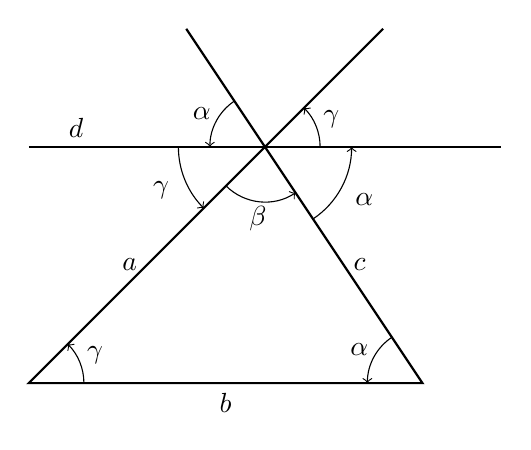
\begin{tikzpicture}[scale=1.0]

	% points
	\coordinate (A) at (0,0);
	\coordinate (C) at (5,0);
	\coordinate (B) at (3,3);

	\coordinate (D) at (4.5,4.5);
	\coordinate (E) at (2,4.5);

	\coordinate (F) at (0,3);
	\coordinate (G) at (6,3);

	% triangle sides
	\draw[thick] (A) -- (B) -- (C) -- cycle;
	\draw[thick] (B) -- (D);
	\draw[thick] (B) -- (E);
	\draw[thick] (F) -- (G);

	% side labels
	\node[left]  at ($(A)!0.5!(B)$) {$a$};
	\node[below] at ($(A)!0.5!(C)$) {$b$};
	\node[right] at ($(B)!0.5!(C)$) {$c$};
	\node[above] at ($(F)!0.1!(G)$) {$d$};

	% angle alpha
	\pic[draw, ->, "$\alpha$", angle eccentricity=1.3, angle radius=0.7cm]
	{angle = B--C--A};
	\pic[draw, ->, "$\alpha$", angle eccentricity=1.3, angle radius=0.7cm]
	{angle = E--B--F};
	\pic[draw, ->, "$\alpha$", angle eccentricity=1.3, angle radius=1.1cm]
	{angle = C--B--G};

	% angle beta
	\pic[draw, ->, "$\beta$", angle eccentricity=1.3, angle radius=0.7cm]
	{angle = A--B--C};

	% angle gamma
	\pic[draw, ->, "$\gamma$", angle eccentricity=1.3, angle radius=0.7cm]
	{angle = C--A--B};
	\pic[draw, ->, "$\gamma$", angle eccentricity=1.3, angle radius=0.7cm]
	{angle = G--B--D};
	\pic[draw, ->, "$\gamma$", angle eccentricity=1.3, angle radius=1.1cm]
	{angle = F--B--A};

\end{tikzpicture}

\end{document}
